\section{Approach and Technical Details}

% TODO: describe the elaboration pipeline
The general approach followed in this class project is based on the one adopted in \cite{Littlewort04dynamicsof,Bartlett06fullyautomatic}, where several concepts and algorithms are mixed and pipelined in order to achieve the not trivial task of the emotional states recognition. The methodology proposed on these papers is the following:

\begin{itemize}
\item Face detection and extraction
\item Facial features extraction via bank of Gabor filters.
\item Training several binary \emph{AdaBoost} classifiers with the labelled data (e.g.\ emotion labels).
\item Extraction of the most relevant features emerged after the training.
\item Most relevant facial features extraction based on valuable features observed.
\item Training several binary \emph{SVM} classifiers with the labelled data (e.g.\ emotion labels), using only most relevant features.
\end{itemize}

During project development we \emph{did not} rigidly follow the pipeline above for several pragmatical reasons, mainly related to the limited amount of time available for the class project. We adopted an approach based on a simplified version of this methodology. In detail our approach is based on the following steps:

\begin{itemize}
\item Face detection and extraction
\item Facial features extraction via bank of Gabor filters.
\item Training several binary \emph{Boost} classifiers with the labelled data (e.g.\ emotion labels).
\item Training several binary \emph{SVM} classifiers with the labelled data (e.g.\ emotion labels).
\end{itemize}

Further detail about reasons that have driven us to this approach can be found in~\ref{res:issues}.\\

In the following paragraphs we resume main characteristics of algorithms and datasets adopted in our class project.

% \cite{Littlewort04dynamicsof}
% \cite{Bartlett06fullyautomatic}
% \cite{learningOpenCV2008}

\subsection{Face Detection}

Face area represent the region of interest (ROI) in the context of this project, so we firstly focused on how to detect faces in an image. This kind of task has been widely discussed in literature and several algorithm implementation exists, in our case we choose to adopt a \code{Haar feature based cascade classifier}\cite{Viola01rapidobject}, which is also part of the OpenCV framework.\\
This detection methodology use an huge amount of simple Haar features to train an \emph{AdaBoost} cascade classifier. In detail the concept involved are:

\begin{description}
\item[Haar Features] this kind of features are calculated in a small windows of the image, in this window a binary mask is virtually applied and the value of the feature is the difference between the sum of the pixel values above the part of the mask with value 1 and the sum of the other part. An example of this kind of feature in fig.\ref{fig:haar}.
\item[Boosting] is a supervised machine learning approach that uses an ensemble of weighted \code{weak classifiers}. Further details in~\ref{appr:boosting}.
\item[Cascade Classification] this classification approach is based on several classification step, in each step a different feature is considered and if a feature value doesn't match the trained model the process is aborted and further stages are not evaluated.
\end{description}

\begin{figure}[!b]
\centering
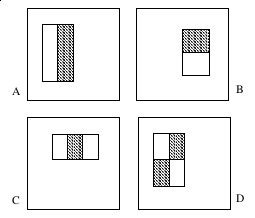
\includegraphics[width=4cm]{images/haarfeatures.png}
\label{fig:haar}
\caption{Haar feature example from \cite{Viola01rapidobject} }
\end{figure}

The OpenCV implementation also support \emph{multiscale detection}, which performs several detection steps rescaling the input image in order to identify object with different size with respect to the training sample sizes. High performance is reached due to the use of the \emph{integral image} for feature calculation. With this approach a single haar-feature can be calculated with 3/4 lookups and a couple of arithmetic operations. The integral image is calculated with the following formula: $ ii(x,y) = \sum_{x' \leq x, y' \leq y}{ i(x',y') } $.\\

However, AdaBoost and Haar features are not the only choice, OpenCV implementation also support \emph{local binary patterns} based features and other boosting algorithms (eg. \code{RealBoost}, \code{GentleBoost}, \code{Discrete AdaBoost}, \ldots).

% \cite{Viola01rapidobject}

\subsubsection*{Face Rotation}

Our projects also implement a simple face rotation correction algorithm, which is based on the position of eyes detected via specifically trained cascade classifiers. Once eyes position is obtained a simple trigonometry calculation is performed in order to get the value of the angle between the eye-line and the x-axis, this value is then used for the definition of rotation matrix which is applied to the whole image.

\subsection{Gabor Filters}

% \cite{gaborTutorial}
% \cite{Lades93distortioninvariant}

\subsection{Boosting}
\label{appr:boosting}
% \cite{rojas2009adaboost}
% \cite{Friedman98additivelogistic}

\subsection{SVM}

% \cite{}

\subsection{Dataset}

% \cite{Kanade2000}

